\documentclass[letterpaper,twocolumn,openany,nodeprecatedcode]{dndbook}

% Use babel or polyglossia to automatically redefine macros for terms
% Armor Class, Level, etc...
% Default output is in English; captions are located in lib/dndstrings.sty.
% If no captions exist for a language, English will be used.
%1. To load a language with babel:
%	\usepackage[<lang>]{babel}
%2. To load a language with polyglossia:
%	\usepackage{polyglossia}
%	\setdefaultlanguage{<lang>}
\usepackage[english]{babel}
%\usepackage[italian]{babel}
% For further options (multilanguage documents, hypenations, language environments...)
% please refer to babel/polyglossia's documentation.

\usepackage[utf8]{inputenc}
\usepackage[singlelinecheck=false]{caption}
\usepackage{lipsum}
\usepackage{listings}
\usepackage{shortvrb}
\usepackage{stfloats}
\usepackage{hyperref}

\captionsetup[table]{labelformat=empty,font={sf,sc,bf,},skip=0pt}

\MakeShortVerb{|}

\lstset{%
  basicstyle=\ttfamily,
  language=[LaTeX]{TeX},
  breaklines=true,
}

\title{Organization}
\author{}
\date{}

\begin{document}

% \frontmatter

% \maketitle

% \tableofcontents

% \mainmatter%

\footnotesize

\begingroup
\DndSetThemeColor[PhbMauve]

\section{Organizations}

% \begin{figure*}
%     \includegraphics[width=\textwidth]{TheUnderworldSyndicate.jpg}
%     \caption{The Underworld Syndicate.}
% \end{figure*}

This book introduces a new level of play; Domain-level play.
The heroes’ domain is called an \textbf{Organization} and the villain’s domain is an \textbf{Enemy Realm}.
NPC domains can be either organization or realm.
Some NPC realms are specific to one ancestry, like a Fae Court or a Dwarven Thanedom!
A Kingdom in this system is just a high level \textbf{Noble Court}. %, one of the 8 different organizations.

% There are many different PC organizations in the book, and each has three specializations.
An organization has a specialization, while an enemy realm does not.
For instance, an \textbf{Underworld Syndicate} is an organization with three different specializations; \textbf{Assassins’ College}, \textbf{Spy Network}, or \textbf{Thieves’ Guild}.
You choose a specialization when you found your organization.
% There are eight organizations each with three specializations, so that’s 24 different kinds of orgs just for players.

% Meanwhile on the other side of the screen, there are 16 more NPC Realms.
% These are self-contained without specializations and cover everything from Giant Jarldoms (a jarldom of giants, not a REALLY BIG jarldom) to Deep Sea Colonies, Draconic Tyrannies and Undead Kingdoms.

% When you see the complete list it should be easy to figure out, regardless of what adventure you’re running, what kind of Enemy Realm your villain is in charge of.
% We want you to be able to use these rules in the game you’re already running, without having to start a new campaign.

The heroes are the \textbf{officers} in their new organization.
If you’re dropping these rules into your existing campaign your organization is probably some version of an \textbf{Adventuring Guild}.
Maybe a Mercenary Company or an Explorers’ Society.

\begin{DndSidebar}{Different Organizations}
  As Kingdoms \& Warfare is \textit{not released yet}, the organizations mentioned in this text are \textit{not yet available}, with the exception of the \textbf{Thieves’ Guild}.
  For the time being I will design the \textbf{Organizations} and \textbf{Enemy Realms} that we need in order to play.
\end{DndSidebar}

\subsection{Adventuring}
% TODO: go over once more

This system assumes that the adventure you’re in the middle of has some kind of Villain or \textbf{Villains}.
They and their \textbf{lieutenants} and \textbf{agents} become an Enemy Realm using these rules, and there’s going to be some kind of climactic final battle between the heroes and the villains.
This should cover most experiences with 5E.

But your characters now have an organization to lead which means while you’re adventuring your organization is using its skills to carry out your orders.
We don’t get too into the details of how exactly your organization knows what you want it to do; whenever your characters get back to civilization they dash off orders and generally \textbf{your NPC lieutenants} know what your goals and intentions are, and can carry them out faithfully while you’re down in a dungeon.
% :D

Eventually your adventuring brings you into \textbf{contact} with the adventure’s villain or their agents, and this means your organization and their organization are now aware of each other ... \textit{and the world isn’t big enough for the both of you!}
\textbf{This is the beginning of the Intrigue.}

\subsection{Intrigue}

Conflict between two domains is called an \textbf{Intrigue}.
Imagine your organization’s agents going out into the world and doing research on the villain’s past to uncover their secrets, sending emissaries to other realms to see which side they’ll be on in the final battle, sending your spies to try to sabotage the enemy’s operations.
All the while, of course, the villain is doing the same thing to you!
This is an \textbf{Intrigue}.

% In the sample adventure, The Regent of Bedegar, the heroes have just taken over Castle Rend in the middle of a forest.
% The nearby noble, Lord Saxton is a villain and an usurper.
% He views the heroes in their new forest fastness as a threat and so vows to crush them.
% Classic!

% Thanks to the heroes’ new Organization and its agents and allies, they know Lord Saxton is planning to raise an army and lay siege to their new fortress.

% Each domain is aware of the other, and each is working to make sure when they finally meet, the battle happens on their terms.

% They’re talking to the Elves and asking for aid against Saxton.
% The Elves say they have no love for the usurper, but their troops are all busy defending their northern border against a Black Dragon.
% “Hmmm...a black dragon you say?”

% You’re fighting a Black Dragon to help the elves, so the elves will lend you aid in your battle against Lord Saxton.

Meanwhile, the heroes are still adventuring!
You’re doing all the same stuff you’d be doing in a normal 5E game, but there’s this added political layer to it.
While you’re collecting allies and aid, your domain takes actions using its skills and abilities, as is the enemy realm. % Lord Saxton’s Despotic Regime (an enemy realm!).

The intrigue ends when your heroes face off against the villain and the results of the intrigue determine the conditions of the battle and which bonuses each side gets in combat and battle.

That’s all pretty high-level and may be hard to picture, so let’s take a look at a sample Organization; the Underworld Syndicate, specifically a Thieves’ Guild.

\pagebreak

\subsection{The Party Sheet}

\begin{figure*}
    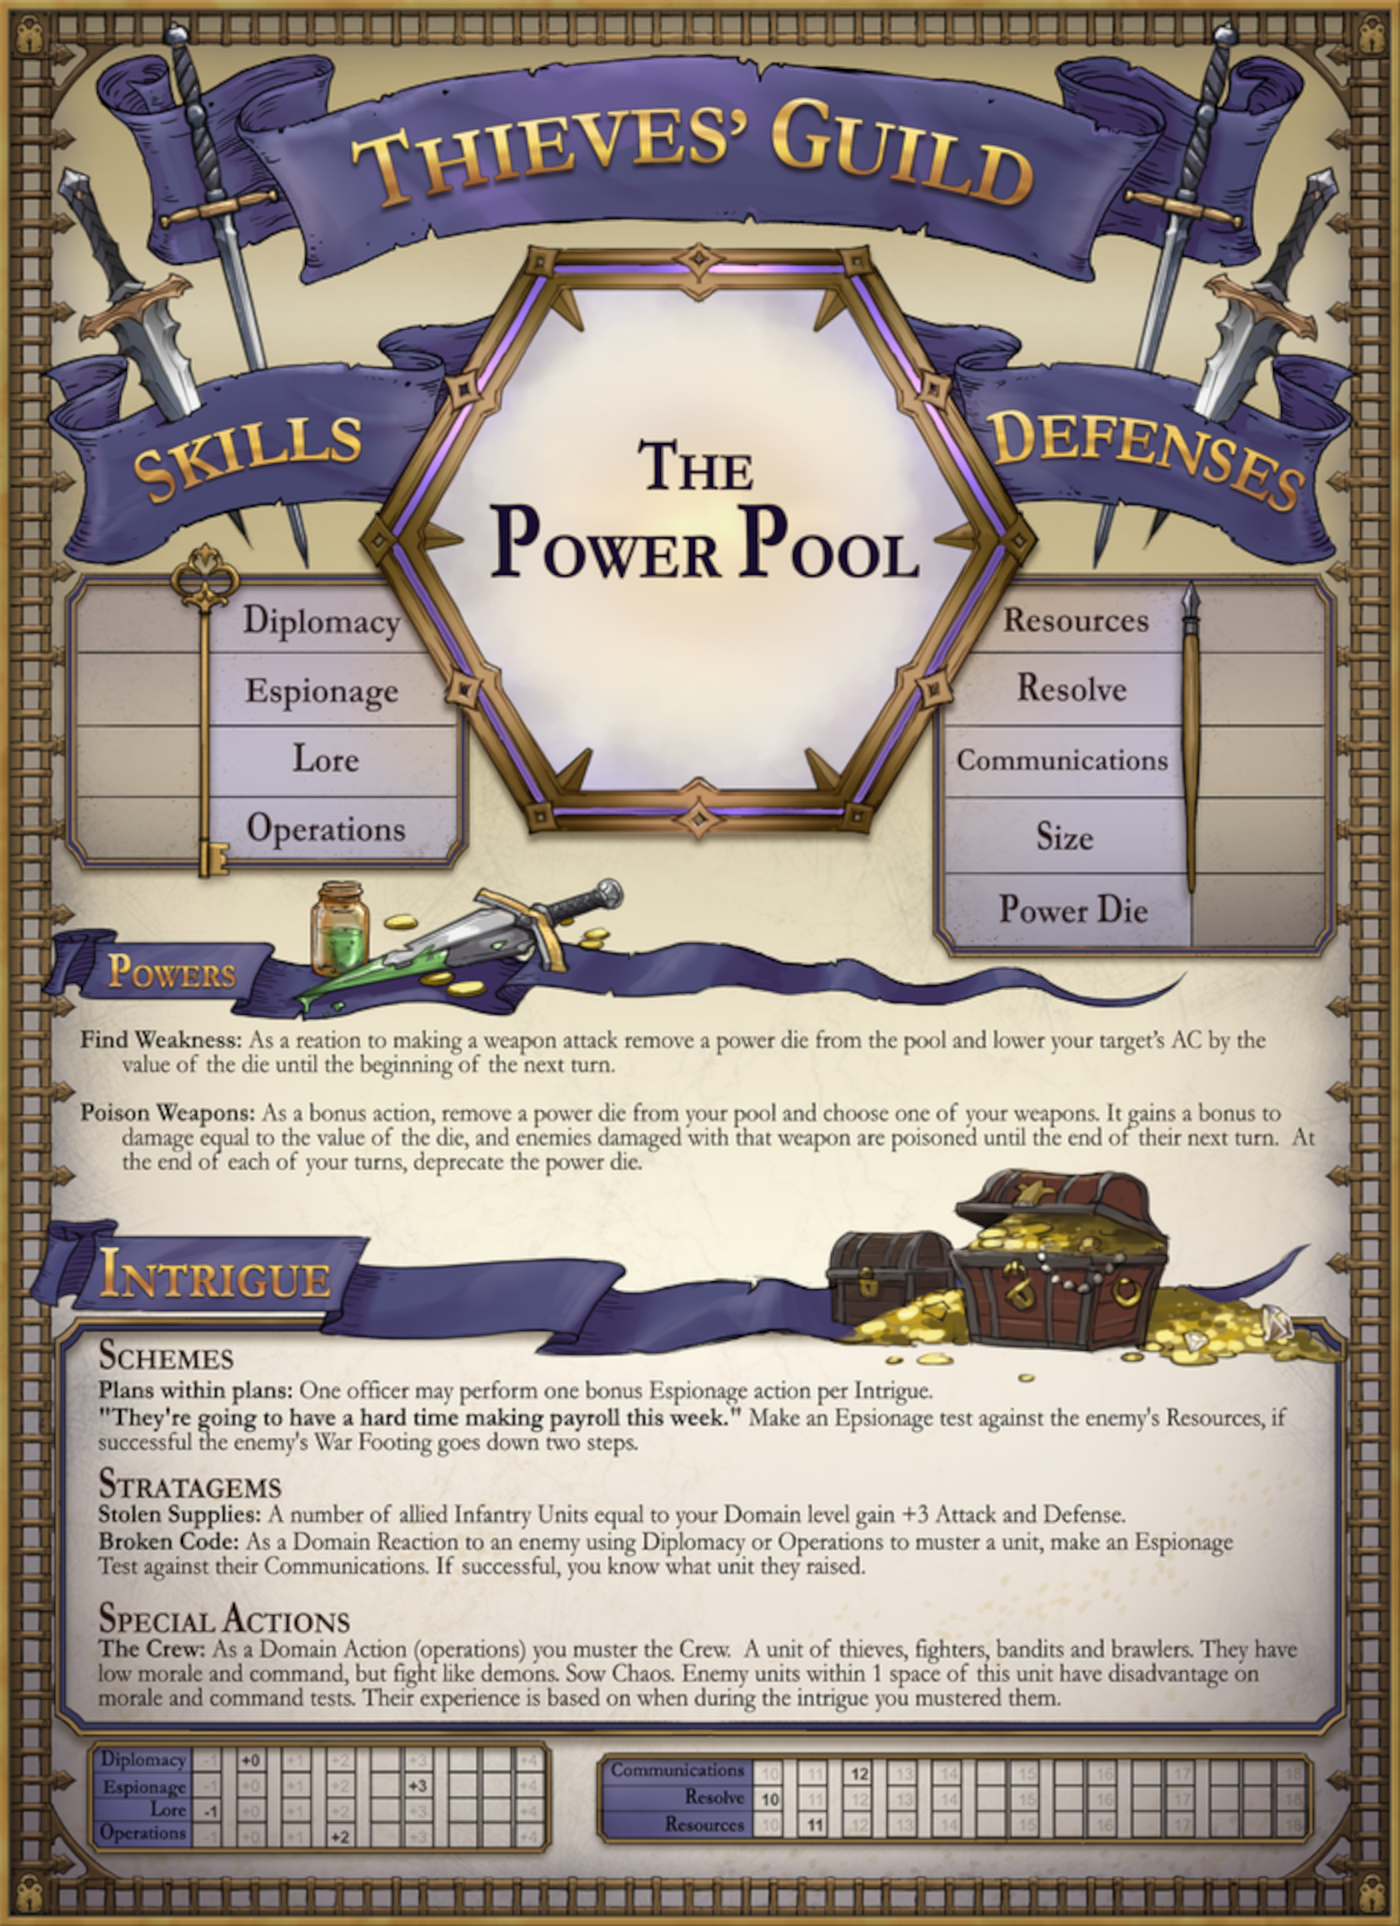
\includegraphics[width=\textwidth]{ThievesGuild.png}
    \caption{Party Sheet of the Thieves’ Guild.}
    \label{fig:org:thieves_guild}
\end{figure*}

Look at Figure \ref{fig:org:thieves_guild}.
This is a Party Sheet.
% Each specialization has one,
It lists all your abilities and also has a little development track to help you when you level up and improve your domain.

You can see the Org has \textbf{four skills}; Diplomacy, Espionage, Lore, and Operations.
It also has \textbf{three defenses}, Communications, Resolve, and Resources.

You can use your org skills the same way you use your character skills.
Outside of intrigue, you can have your agents negotiate with nearby realms (diplomacy) or dig into another realm’s secrets (espionage), you can research deep history or obscure magical knowledge (lore) or do mundane things like build roads or cultivate farmland (operations).

During Intrigue your domain gets a number of actions based on its level.
A domain action uses a skill and targets either a listed DC or another realm’s defenses.
If you’re negotiating with the Elves to get their help against Lord Saxton, the DC for your Diplomacy test is set by the \textbf{Attitude} of the NPC Realm.

Each realm, including yours, also has \textbf{three Readiness levels} that describe how prepared you are for the upcoming combat or war.
Each Readiness level grants your benefits in combat or battle.

You can use your actions to raise your Readiness or lower the enemy’s Readiness.
You can make an \textbf{Operations} test to raise new units, but you may want to make an \textbf{Espionage} test first to see which units the enemy has!
You can also use your \textbf{Diplomacy} to recruit Allied Units from local NPC Realms.

% If you’re trying to sabotage Lord Saxton’s plans using your Espionage, you choose a Defense and make a roll.
% Success lowers one of Lord Saxton’s Readiness levels which means he and his lieutenants or soldiers begin the final combat with a penalty.

\textit{Which skill you use, which defense you target, and which readiness level you raise or lower is up to you.}
The goal is to let the players \textbf{be creative}.
As long as the GM agrees their plan is reasonable, they can try it.
But the GM might feel like, based on what the heroes are trying, this action would target the enemy’s Resolve rather than Communications, for instance.
The players invent a plan, but the GM gives feedback on what they think is reasonable.

\subsection{Customizing Your Org}

\begin{table}
    \begin{DndTable}[]{XXXX}
        \textbf{Size (Level)} & \textbf{Power Die} & \textbf{Development Points} & \textbf{Points per player} \\
        1         &  1d4 & 16 & 4 \\
        2         &  1d6 &  8 & 2 \\
        3         &  1d8 &  8 & 2 \\
        4         & 1d10 &  8 & 2 \\
        5         & 1d12 &  8 & 2 \\
    \end{DndTable}
    \caption{Leveling Table assuming Four (4) Players.}
    \label{tab:org:leveling}
\end{table}

As you can see, the bottom of the sheet starts with some values already printed on the sheet for each skill and defense based on what that Organization is good at, and how that Specialization modifies things.
An Underworld Syndicate is good at Espionage!
But a Thieves’ Guild is a kind of Underworld Syndicate that’s also good at Operations.

After you choose your organization, the players each get a \textbf{four Development Points} to spend customizing their organization.
And two more each level above the first.
You (literally) pass the sheet around the table, with each player using one point to mark off one box, until all players have spent all their points.

This is the beginning of feeling like an organization.
Like a team.
You may not all agree on how to spend your points!
You have to cooperate, communicate, and maybe compromise.
Yes, you may argue about whether your Knightly Order should be better at Diplomacy or Lore.
You may not agree.
That’s part of the point.
One way or the other, you have to work together.
% :D

\subsection{Schemes \& Stratagems}

Each org gets two abilities that help it during Intrigue and these are called \textbf{Schemes} along with two abilities that help it during Warfare, called \textbf{Stratagems}.
You get one Scheme and one Stratagem from your org and one from your specialization.

Schemes and stratagems are fun abilities that not only give you more options, but also help make your org feel unique and reinforce the fantasy of “we are a thieves’ guild” or “we are an arcane order.”

But I think the star of the show is the new Powers you get!

\subsection{Powers}

\textbf{Powers} are the benefits your characters get for running an organization.
They represent the idea that \textit{you’re no longer a disparate group of random weirdos, \textbf{you are now a team}} and gain special benefits because you’ve been working together and training together and you’ve learned all sorts of cool tricks and ways to synergize your abilities.

% Imagine the X-Men and all the crazy tricks and tactics they’ve developed together that none of them could do alone.
% The Fastball Special.
% Or the Fellowship of the Ring learning how to work together in ways they couldn’t do without practice adventuring together.
% These are your Organization Powers.

Each \textbf{officer} gets a die, the \textbf{Power Die}.
The size of the die is determined by the level (aka the size) of your organization.

At the start of the final battle with the leader of the Enemy Realm (aka the villain of this adventure, or the miniboss of this chapter) all the officers in your org roll their Power Die and place the die, with its result showing, in the Power Pool on the Party Sheet.

Then, during the final battle, any officer can use these dice on their turn to perform the listed action.
Some powers use one die, or several.
Some use all the dice!

Of course, the villains’ realm also has powers!
If you use these rules, the final battles of your adventures feature more...pyrotechnics.
% :D

\subsection{Special Actions}

Each org may also get one or more special actions, things only your domain can do.
Usually this is about raising unique units.
Only a Thieves’ Guild can raise The Crew for instance, a unit of fighters, thieves, bandits, and brawlers.

\subsection{Resolving Intrigue}

The intrigue ends after both domains have taken all their actions and prepare for the Final Battle which is probably a normal Boss Fight, just with cool powers and probably a battle happening at the same time.

Each domain has three categories of Readiness, their \textbf{War} Readiness, their \textbf{Combat} Readiness, and the \textbf{Intel} they’ve gathered.
Over the course of the intrigue you’re using your actions to boost your readiness, and lower your enemies.
Each Readiness level grants bonuses to the combat or the battle but they are undergoing a revision right now and I want the testers to try out the new Readiness levels before I share them.

Each of these systems is designed to be optional.
You could plunder this book and only use the Powers, so now your party has these cool new abilities, but you have to communicate and work together to get the maximum value from them.

Or you could just use the Org Skills and Defenses and run a game very like a normal 5E game, but with added political sophistication thanks to these rules.

Likewise, the Warfare system is designed to be used parallel to the Final Battle of an adventure, but we’ve designed and tested it to make it fun and robust to use to fight a war all by itself!
Speaking of which....

\pagebreak

\section{TL:DR}

\subsection{Size \& Power Die}
The \textbf{Size} of your organization represents its \textbf{Level}, it reaches from 1 to 5.
Your \textbf{Power Die} increases with each level up. See Table \ref{tab:org:leveling}.
\textbf{Development Points} can be used to increase your orgs Skills and Defense, bottom of thr Party Sheet (Figure \ref{tab:org:leveling}).

\subsection{Skills}
The \textbf{Skills} of an organization are used just like normal D\&D 5e Skills from a Character.

\paragraph{Diplomacy} describes your orgs ability to negotiate with other organizations or realms.

\paragraph{Espionage} is used to \textbf{spy} on other organizations and \textbf{gather current information}.

\paragraph{Lore} can be used to uncover \textbf{historic} and sometimes \textbf{arcane knowledge}.

\paragraph{Operations} describes your orgs ability to \textbf{muster units}, \textbf{transport resources} and \textbf{organize itself} in a effective and efficient fashion.

\subsection{Defenses}

\paragraph{Communications} describes how difficult it is to \textbf{gather intel on you} and your plans.
\textit{How well protected is the communication between the officers (you), your lieutenants (retainers), and other organization members (units and others).}

\paragraph{Resolve} is a vital part of your org. To keep your subordinates in line, their resolve must not be attacked.
% TODO: ehhh

\paragraph{Resources} Every org needs resources in order to function. \textbf{Intrigue} and \textbf{Warfare} must be \textbf{financed}. People need to eat, sleep, and get paid.

\subsection{Readiness}
The \textbf{Readiness} of an organization describes its ability to face another.
There are \textbf{three} types of Readiness.

\textbf{War Footing} describes the ability of an organization to conduct \textbf{Warfare}.
% TODO: what exactly does this do?
% reduce the number or units?
% reduce the equipment bonus?
% give units disadvantage?

\textbf{Combat Preparations} describes the ability of an organization to engage in \textbf{Combat}.
% TODO: what exactly does this do?
% surprise round?
% less enemy creatures / minions
% does not get legendary actions in first round?
% does not get lair actions in first round?

\textbf{Intel} describes the amount and quality of information an organisation gets in order to prepare for the upcoming confrontation.
An organisation may conduct preparations based on that information.
% For example, a spell casting heavy party may find their enemy deploying \textit{counterspell}.

% \begin{DndSidebar}{Unfinished Design}
%   As the Readiness Desgin is not yet finished.
%   I will probably default to only one (1) Readiness value to keep it simple.
% \end{DndSidebar}

\subsection{Intrigue}
An \textbf{Intrigue} is managed similar to a combat encounter in the sense of rules.
It consists of multiple rounds and each organization gets actions based on its level.
Opposed to combat however, it takes place over an extended period of time.
One round might be as long as one month, depending on your game.

\paragraph{Actions} can be a \textbf{Skill check} targetting a \textbf{Defense} or one of the actions below.

\paragraph{Schemes} are \textbf{Intrigue Actions} focused on political goals.
They usually targetting the \textbf{Readiness} of an enemy organization.
Each organization has \textbf{two (2)} of them.

\paragraph{Stratagems} are \textbf{Intrigue Actions} focused on Warfare.
Each organization has \textbf{two (2)} of them.

\paragraph{Special Actions} usually muster a \textbf{special unit}.
Each org has at least \textbf{one (1)}.

\pagebreak

\section{Credits}

This material is for personal use only.
As it is based on non-free material, released as a \href{https://www.kickstarter.com/projects/255133215/kingdoms-warfare-and-more-minis/posts/3002949}{Design Update} for Kingdoms \& Warfare written by \textbf{Mathew Colville}.

However this document also includes \textbf{homebrew additions} to the system presented by MCDM in order to fill up some unfinished parts and make it playable.
These additional rules where created by \textbf{Jens Keim}.
The additional rules can be used under the \textbf{OGL v1.0a}.
And flavor and description texted is released under \textbf{CC-BY-SA-4.0}

Everything not included in the public post linked above is therefore free to be shared under the appropriate licenses.

\subsection{Sources}

\url{https://www.kickstarter.com/projects/255133215/kingdoms-warfare-and-more-minis/posts/3002949}

\section{Dungeon Master}

As a \textbf{Dungeon Master} you manage the NPC Organizations and Enemy Realms.

If you want to design your own organization you can use the the following rules. % based on the example organization we know so far.
An organization starts with 12 \textbf{Development Points}.
The \textbf{Thieves Guild} has 9 placed in skills and 3 in Defenses.
The \textbf{Organization Type} provides the best skill (5 points) and defense (2 points), while the \textbf{Specialization} gives us the second best skill (3 points) and defense (1 point).
This reasoning is based on the following lines of Matts announcement and I think it is a safe path to follow for basic organization design.

\begin{DndReadAloud}
    An Underworld Syndicate is good at Espionage!
    But a Thieves’ Guild is a kind of Underworld Syndicate that’s also good at Operations.
\end{DndReadAloud}

The remaining 1 point in our example, the Thieves' Guild, is placed in any skill, but one could as easily place it in a defense instead.
Feel free to change it up.
I'd suggest using at least 3 on each side, offense and defense, and than place the others as you see fit.
However there is no reason to limit the DM to this, so if you think something else would be cool and balanced go for it.

Besides the \textbf{base} Development Points there are also 11 \textbf{extra Development Points} the DM can distribute to the players for cool roleplaying moments in scenarios that relate to the organization, either political or warfare related.
Just keep in mind, if you let the organization levels fast and you distribute all the extra points your players will have a maxed out organization, or \textbf{Legendary Organization} as I like to call it, sooner rather than later.

\begin{table}
    \begin{DndTable}[]{XXXX}
        \textbf{Size (Level)} & \textbf{Power Die} & \textbf{Development Points} & \textbf{Accumulative Points} \\
        base      &    - & 12 & 12 \\
        1         &  1d4 & 16 & 28 \\
        2         &  1d6 &  8 & 36 \\
        3         &  1d8 &  8 & 44 \\
        4         & 1d10 &  8 & 52 \\
        5         & 1d12 &  8 & 60 \\
        extra (6) & 1d20 & 11 & 71 \\
    \end{DndTable}
    \caption{Leveling Table for DM}
    \label{tab:org:leveling_dm}
\end{table}

\end{document}
